% Figure 4: Evaluation Results - Violation Distribution and Performance
% Author: OTLP Project
% Date: October 20, 2025

\begin{figure}[t]
\centering

% Left subplot: Violation Distribution
\begin{subfigure}[b]{0.48\columnwidth}
\centering
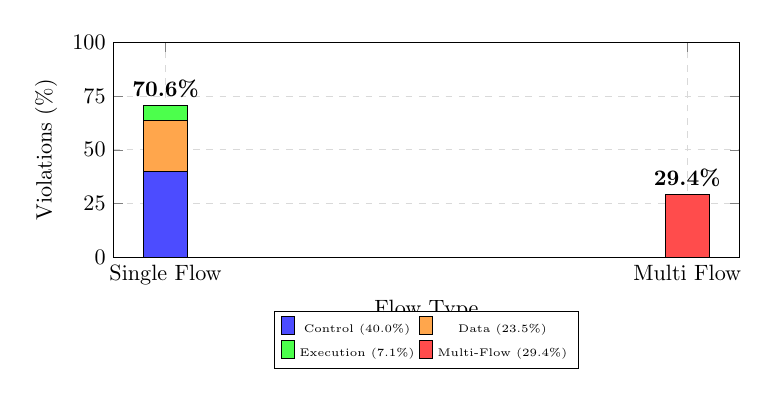
\begin{tikzpicture}[scale=0.8]
\begin{axis}[
    ybar stacked,
    bar width=20pt,
    ylabel={Violations (\%)},
    xlabel={Flow Type},
    ymin=0, ymax=100,
    xtick=data,
    xticklabels={Single Flow, Multi Flow},
    ytick={0,25,50,75,100},
    legend style={at={(0.5,-0.25)}, anchor=north, legend columns=2, font=\tiny},
    width=0.95\columnwidth,
    height=5cm,
    grid=major,
    grid style={dashed, gray!30}
]

% Single flow stack
\addplot[fill=blue!70, draw=black] coordinates {(0,40.0) (1,0)};
\addplot[fill=orange!70, draw=black] coordinates {(0,23.5) (1,0)};
\addplot[fill=green!70, draw=black] coordinates {(0,7.1) (1,0)};

% Multi flow
\addplot[fill=red!70, draw=black] coordinates {(0,0) (1,29.4)};

\legend{Control (40.0\%), Data (23.5\%), Execution (7.1\%), Multi-Flow (29.4\%)}

% Add total labels on bars
\node[above] at (axis cs:0,70.6) {\textbf{70.6\%}};
\node[above] at (axis cs:1,29.4) {\textbf{29.4\%}};

\end{axis}
\end{tikzpicture}
\caption{Violation distribution}
\label{fig:eval-violations}
\end{subfigure}
\hfill
% Right subplot: Performance Breakdown
\begin{subfigure}[b]{0.48\columnwidth}
\centering
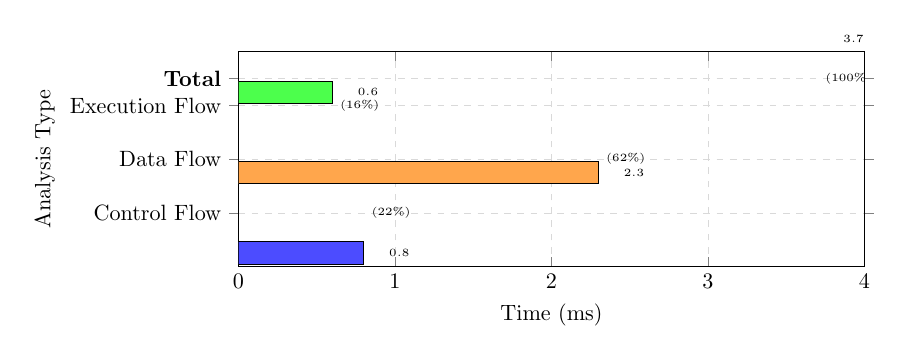
\begin{tikzpicture}[scale=0.8]
\begin{axis}[
    xbar,
    bar width=10pt,
    xlabel={Time (ms)},
    ylabel={Analysis Type},
    ymin=0, ymax=4,
    xmin=0, xmax=4,
    ytick={1,2,3,3.5},
    yticklabels={Control Flow, Data Flow, Execution Flow, \textbf{Total}},
    xtick={0,1,2,3,4},
    width=0.95\columnwidth,
    height=5cm,
    grid=major,
    grid style={dashed, gray!30},
    nodes near coords,
    nodes near coords align={horizontal},
    every node near coord/.append style={font=\tiny, xshift=8pt}
]

\addplot[fill=blue!70, draw=black] coordinates {(0.8,1)};
\addplot[fill=orange!70, draw=black] coordinates {(2.3,2)};
\addplot[fill=green!70, draw=black] coordinates {(0.6,3)};
\addplot[fill=gray!70, draw=black, thick] coordinates {(3.7,3.5)};

% Percentage annotations
\node[right, font=\tiny] at (axis cs:0.8,1) {(22\%)};
\node[right, font=\tiny] at (axis cs:2.3,2) {(62\%)};
\node[right, font=\tiny] at (axis cs:0.6,3) {(16\%)};
\node[right, font=\tiny] at (axis cs:3.7,3.5) {(100\%)};

\end{axis}
\end{tikzpicture}
\caption{Performance breakdown}
\label{fig:eval-performance}
\end{subfigure}

\vspace{0.3cm}

% Bottom: Key Statistics
\begin{center}
\begin{tabular}{|l|c|c|c|}
\hline
\textbf{Metric} & \textbf{Value} & \textbf{Dataset} & \textbf{Complexity} \\
\hline
Total Traces & 9.3M & Production & - \\
Violations Found & 255K (2.74\%) & Real-world & - \\
\textbf{Multi-Flow} & \textbf{75K (29.4\%)} & \textbf{Critical} & - \\
Avg Time/Trace & 3.7ms & Rust impl. & $O(|N|^2 \times |A|)$ \\
\hline
\end{tabular}
\end{center}

\caption{Evaluation results on 9.3M production traces. \textbf{(a)} Violation distribution showing 70.6\% single-flow violations (Control: 40.0\%, Data: 23.5\%, Execution: 7.1\%) and \textbf{29.4\% multi-flow violations} that require integrated analysis. \textbf{(b)} Performance breakdown showing 3.7ms average verification time per trace, with Data Flow analysis dominating (62\%, 2.3ms) due to $O(|N|^2 \times |A|)$ complexity for context and attribute propagation. The high proportion of multi-flow violations validates our integrated Triple Flow approach—single-perspective analysis would miss nearly one-third of protocol violations.}
\label{fig:evaluation}
\end{figure}

